\chapter{O Texto da Tese}

O texto da tese (ou dissertação) é de responsabilidade única do candidato. Claramente, o orientador deve orientar a direção desse texto, mas o responsável único, aquele que será aprovado em função do texto, é o aluno.

Não é função do orientador corrigir o português (ou inglês) dos alunos; ao contrário, como orientador, eu espero que os alunos possuam um português de qualidade. Se seu português é ruim, procure um revisor, seja um amigo ou parente voluntário, seja um profissional que você terá que pagar.

Os alunos de doutorado devem priorizar escrever sua tese em inglês. Os alunos de mestrado devem tentar.

\CoppeWay{Línguas Usadas na Tese}{
Na Coppe o texto pode ser em português, inglês ou espanhol. Outra língua pode ser usada, mas precisa ser autorizada.
}

\needspace{5\baselineskip}
\section{7 Capítulos }
O número místico 7 aparece aqui para definir o número de capítulos da sua tese, que tem normalmente a seguinte estrutura (meus alunos):
\begin{enumerate}
\item	Introdução: incluindo motivação, introdução ao tema, premissas, questões de pesquisa ou hipótese, objetivos e metas, descrição dos próximos capítulos
\item	Revisão do Problema: incluindo áreas relacionadas, de preferência por meio de Revisão ou Mapeamento Sistemático, em formato top-down, do problema mais geral ao mais específico.
\item	Revisão das Técnicas de Solução ou Metodologia: mostrado, de forma top-down, as teorias, técnicas, tecnologias ou metodologias usadas na solução do problema
\item	Proposta de Solução: na forma teórica ou conceitual
\item	Implementação: descrição da arquitetura e detalhes técnicos
\item	Experimentos: incluindo resultados e comentários
\item	Conclusão: incluindo contribuições gerais (melhoria na solução de um problema) e específicas (bibliotecas de código) e trabalhos futuros.
\end{enumerate}


Isso pode ser reduzido para 5 capítulos:
\begin{enumerate}
    \item	Introdução
   \item	Revisão
   \item	Proposta
   \item	Experimentos
   \item	Conclusão
\end{enumerate}

É curioso que devido a uma superstição iniciada por um professor da PUC que era ligado à numerologia e outras coisas místicas, evitamos teses com 6 capítulos, um número que não é de sorte!

\needspace{5\baselineskip}
\section{Uma estratégia de escrita}

A tese, ou dissertação, é uma descrição do seu trabalho. Uma boa estratégia para fazer essa descrição é partir das perguntas 5W2H.

Primeiro faça uma lista do que você fez (What).

A partir dessa lista, pergunte para cada coisa que você fez: por que você fez (Why) e como você fez (How).

Isso permitirá gerar um mapa de tudo que deverá aparecer na sua tese.

Quando falo em mapa, digo de forma abstrata, porém não é má ideia construir um mapa conceitual de tudo isso.

As outras perguntas (Where, Who, When, How Much) são menos importantes nesse caso, mas podem dar ideias de trabalho. Por exemplo, onde você fez alguma mudança no código? Quem foi o idealizador de algum algoritmo que você uso? Quanto poder computacional você precisou usar?

Você também pode pensar em 2 Whats: qual o seu problema, qual o seu trabalho. E depois fazer um raciocínio similar. A Figura a seguir mostra uma esquema de raciocínio.

% TODO: \usepackage{graphicx} required
\begin{figure}[hbt]
    \centering
    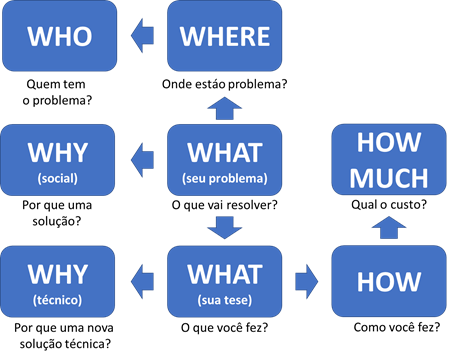
\includegraphics[width=0.7\linewidth]{Images/5w2h}
    \caption{Perguntas que devem ser respondidas antes de iniciar uma tese. Fonte: do autor.}
    \label{fig:5w2h2}
\end{figure}

\section{A tese está no passado}

A tese descreve um trabalho feito. O tempo básico dela é o passado,\textbf{ pretérito perfeito}. Normalmente, o autor não se refere a si, e se o faz, é em um momento onde isso é importante. Em português é comum usar a voz passiva e o sujeito indeterminado, mas a voz passiva não é considerada boa forma em inglês. Nunca usar a primeira pessoa do plural, o ``nós'', que é majéstico, para se referir apenas a você.

O texto, porém, se refere a si mesmo no presente. O presente também é usado para descrever o estado atual das coisas. No texto a seguir, mostramos que a tese ``apresenta'', no presente, trabalhos feitos no passado (``iniciou'',``levou'', ``chegou'') e tem uma proposta de trabalho futuro (``terá'').

\begin{quote}
Esta tese \textbf{apresenta} uma proposta para calcular o número de átomos no universo. Para isso, \textbf{iniciou}-se o processo com uma conta no guardanapo, que \textbf{levou} a diversos experimentos realizados ao longo de dois anos. No final, \textbf{chegou}-se à conclusão de que essa conta será sempre uma estimativa e que a matéria escura ainda \textbf{terá} que ser estimada de forma mais eficaz.
\end{quote}

\needspace{5\baselineskip}
\section{Quanto às figuras}

As figuras ilustrativas de todos os trabalhos dos alunos devem ser feitas, sempre que isso for possível, em linguagens gráficas com uma definição clara\footnote{Fluxogramas são uma linguagem específica, e não um amontoado de caixas e fluxos, que não devem mais ser usados, já que é uma linguagem antiga.}. 

A língua franca da computação atual é UML, que possui uma quantidade de diagramas que ainda podem ser especializados por meio de estereótipos. Outras linguagens podem ser características de áreas específicas, como BPMN e ARIS na descrição de processos de negócio. Deve ficar claro que um gráfico que não é baseado em uma linguagem padronizada, na prática, não significa nada, e passa a ser apenas uma ilustração.

% TODO: \usepackage{graphicx} required
\begin{figure}[hbt]
    \centering
    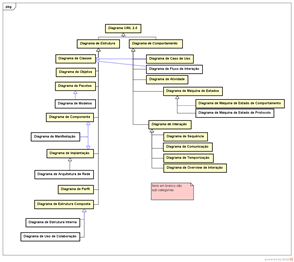
\includegraphics[width=0.7\linewidth]{Images/diagramasuml}
    \caption{Diagramas UML. Fonte: OMG}
    \label{fig:diagramasuml}
\end{figure}





